If you make a big document, for example a book which has more than 100 pages, then using rake is not a good way to test-compile.
The bigger the dicument is, the longer time the compiling takes.

It is a better way to use `lb' to test-compile a subfile separately.
Lb makes a temporary rootfile which includes only the subfile and compile it once.
The advantage of this way is very quick to compile.
However, it has disadvantages.
It only compiles the subfile, so the pdf you get is not a finished document.
It compiles once, so cross-reference doesn't work at all.
It is difficult to say which is better.
it depends on the size of your document.
If it is very big, use lb to test-compile separately.

In this section, I want to show you how to use lb to test-compile a subfile.
This document `Tutorial' is not big, but it's OK.
This is an example to show how to use lb.

Type the following.
\begin{verbatim}
$ lb installation
\end{verbatim}
The argument is a subfile.
The suffix can be left out.
Then, lb makes a temporary rootfile `\_build/test\_installation.tex'.
Its preamble is a copy of the preamble in the original rootfile.
It has {\textbackslash}input command and includes the subfile `installation.tex'.
Lb compiles `\_build/test\_installation.tex' and run the previewer specified in `lb.conf' to show the pdf.
\begin{center}
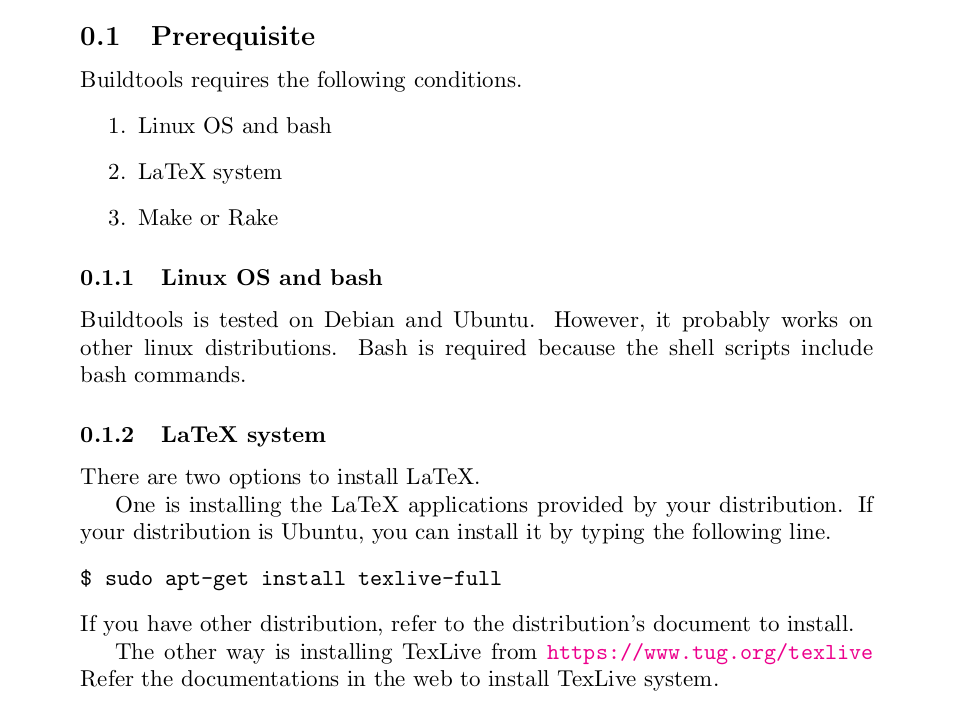
\includegraphics[width=12cm]{test_installation.png}
\end{center}

Lb compiles a subfile with the option synctex on.
Therefore, if you open the source files, `\_build/test\_installation.tex' and `installation.tex' in this example, you can do forward search and backward search between the source and pdf.
If your use gedit and evince, backward search works by clicking left button with pressing down CTRL key, but forward search from `installation.tex' doesn't work.
If you want to do it, add the following line at the beginning of the subfile.
\begin{verbatim}
% mainfile: _build/test_installation.tex
\end{verbatim}
However, forward search isn't used so often compared to backward search.
Adding the line above is usually unnecessary.

